% !TEX root =../main.tex

\chapter{Auswahl an Konzepten Festlegen}


\section{Voraussetzung bei der Entwicklung}


\subsection{Stickiness zwischen Nutzer und Webseite verstärken}

% TODO: Vollständigen Namen des Institus Nielsen angeben. Vielleicht als Fußnote.
% TODO: Genaues Datum angeben bei `Nielsens am Dienstag veröffentlichte ...'
% TODO: Bitte wörtliches Zitat auf Korrektheit überprüfen: `ist drei Viertel der Online-Nutzer auf der Welt zugreifen können.'
% TODO: Genauen Zeitraum angeben bei `haben im vergangenen Monat ...'. Besser ist `haben im Mail 2018 ...'.

Laut dem Marktforschungsunternehmen Nielsen verbringen Nutzer mit Instant Messaging, dem Schreiben von Kommentaren, Bloggen, Teilen und \glqq{}Liken\grqq{} durchschnittlich 22\% ihrer Online-Zeit. Eine durch Nielsen veröffentlichte Statistik zeigte, dass Menschen alle 4,5 Minuten ihrer Online-Zeit eine Minute in sozialen Netzwerken verbringen. Internetnutzer verbringen somit jeden Monat 110 Milliarden Minuten in sozialen Netzwerken und Blogs. Die Umfrage sagt, dass dies das erste Mal ist, dass auf ein soziales Netzwerk oder einen Blog \glqq{}drei Viertel der Online-Nutzer auf der Welt zugreifen.\grqq{} Das ist eine Steigerung von 24\% gegenüber dem gleichen Zeitraum des Vorjahres. Die beliebtesten Social-Networking-Marken sind Facebook und YouTube. Online-Nutzer haben im vergangenen Monat 13 Milliarden Videos auf YouTube gesehen. Facebook meldete, dass seine Nutzer 2 Milliarden Videos pro Monat sehen.

% TODO: (Nielsen-Studie: Facebook und Google haben erfolgreichste Apps Jonas Wagner) in litertur.bib einfügen. `

Laut Nielsens Studie hat Facebook in den globalen Online-Stunden das Rampenlicht übernommen. Fast 500 Millionen Nutzer verbringen jeden Monat sechs Stunden damit.
Was die Netzabdeckung betrifft, übernimmt Google die Führung. Laut Nielsen-Statistiken besuchen 82\% der Internetnutzer weltweit jeden Monat diese Website, und die durchschnittliche Suchzeit beträgt 1 Minute und 20 Sekunden.(Nielsen-Studie: Facebook und Google haben erfolgreichste Apps Jonas Wagner)

D. h. die Zeitdauer, welche ein Nutzer auf einer Webseite verbringt, ist ein Zeichen dafür, ob diese Webseite beliebt ist und ob die User Stickiness stark ist.

Ein wichtige Frage bei dem Entwurf einer Webseite ist, wie man Nutzer motiviert, mehr Zeit auf dieser Webseite zu verbringen. Durch interessante Funktionen und Veranstaltungen?


\subsection{Online Shops welche mehr Produkte verkaufen sind beliebter}

Nach der Statistik von Alexa in Abbildung \vref{fig:alexa}, sind die Top 10 Webshops mit dem höchsten Umsatz unter anderem Amazon, Netflix, Ebay, Walmart, Etsy, Steam und Ikea. Sie alle haben eine Gesamtheit: Es ist eine hohe Vielfalt an Produkten verfügbar.

\begin{figure}
	\centering
	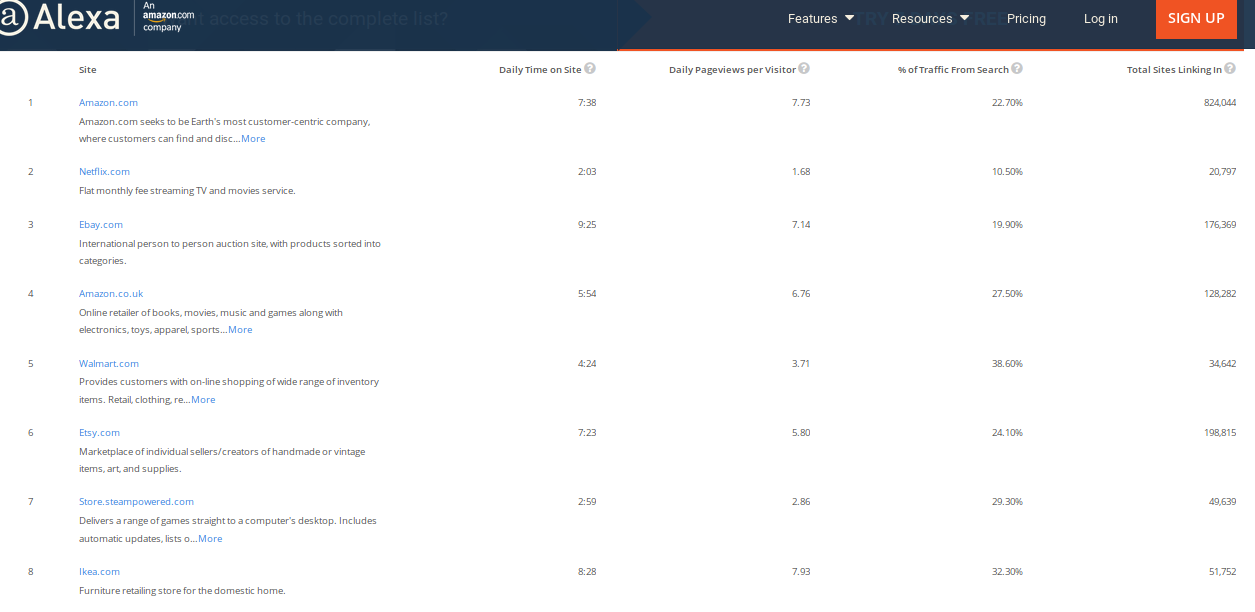
\includegraphics[width=1\textwidth]{bilder/alexa.png}
	\caption{Alexa}
	\label{fig:alexa}
\end{figure}


\section{Freunde organisieren}

Man verwendet Listen, um  Freunde zu organisieren. Mit einer Liste kann man die Meldungen in seinem News-Feed filtern oder Aktualisierungen mit bestimmten Personen teilen. Z. B. mit Arbeitskollegen oder Freunden, die in der Nähe wohnen. Man kann jederzeit Freunde hinzufügen order entfernen. \parencite{facebook:help}

\textbf{Enge Freunde:} Freunde, mit denen man möglicherweise alles teilen möchte.

\textbf{Bekannte:} Personen, mit denen man eventuell weniger teilen möchte.

\textbf{Eingeschränkt:} Diese Liste ist für Personen, die man als Freunde hinzugefügt hat, mit denen man aber nichts teilen möchte. Z. B. einem Arbeitskollegen oder Vorgesetzten.

Man kann außerdem selbst definierte Listen erstellen,  um selbst Freunde in Gruppen zusammenzufassen. Der Nutzer legt fest, wer zu einer bestimmten Liste hinzugefügt wird und welche Privatsphäre-Einstellungen (gegebenenfalls) gelten. Es ist zu beachten, dass Freunde nicht benachrichtigt werden, wenn sie zu benutzerdefinierten Listen hinzufügt werden.


\section{Echtzeitkommunikation mit anderen Nutzern, Verkäufern und dem Kundenservice der Plattform}

Ein potentieller Nachteil von Amazon ist, dass es schwer ist mit dem Verkäufer oder dem Kundenservice persönlich in Kontakt zu treten. Dadurch kann das Kommunizieren und Lösen von Problemen zeitaufwändig und kompliziert ausfallen.

Durch die Verwendung von Echtzeit-Kommunikation, können Probleme unter Umständen deutlich schneller und unkomplizierter gelöst werden. Dies könnte das Einkaufserlebnis deutlich verbessern.


\section{Offline Kontakte}

Eine URL als Nachricht per E-Mail und SMS versenden, welche die Produktinformation beinhaltet. Freunde oder Bekannte müssen sich so nicht noch einmal anmelden, sonder können direkt die URL anklicken. Dadurch werden sie automatisch in die Bestehende Sitzung des Käufers eingeloggt und können sofort Vorschläge unterbreiten und bei der Entscheidungsfindung unterstützen.


\section{Share und Like}

In der zu konzipierenden Webseite soll ein spezieller Platz angeboten werden, an dem Nutzer Erfahrungen oder Kommentare teilen können. Bevor potentielle Kunden eine Kaufentscheidung treffen, können sie die Erfahrungen und die Nachnutzungseffekte anderer Personen nutzen.


\section{Pay by others}

Wenn ein Kind die finanzielle Hilfe der Eltern benötigt, können sich die Eltern auch in dem genutzten Webshop einloggen und entscheiden, ob sie für die Produkte des Kindes bezahlen wollen.


\section{Zusätzliche Services}


\subsection{Weitere Entwicklungen auf der Basis von eBay Kleinanzeigen}

Von eBay Kleinanzeigen zum online Flohmarkt.

Gebrauchte Produkte werden auf der Webseite angezeigt. Die Produkte werden nicht mehr nach einzelnen Attributen klassifiziert, sondern werden gemäß ihrem Verkäufer gruppiert. Ähnlich wie bei dem Besuch eines Flohmarktes. Die gebrauchten Produkte werden nicht nach Attributen sortiert aufgestellt. Z. B. werden nicht alle Spielzeuge des Flohmarkts an einer Stelle verkauft, sonder die Produkte sind nach ihrer Quelle, ihrem Verkäufer sortiert.


\subsection{Communities  für die Nutzer erstellen, um Nachrichten zu veröffentlichen und Erfahrung auszutauschen}

\begin{itemize}
\item Kooperation existiert vor allem in Computerspielen
\item Darstellung und Interaktion im Webshop wird denen von Computerspielen nachempfunden
\item 3D Darstellung und Steuerung wie in Computerspielen
\end{itemize}


\section{Nutzer-Community}

Nutzer- Community dient dazu die Tipps und das Feedback vor und nach dem Kauf zu teilen. Unabhängig vom Preis einer Ware werden Menschen vor dem Kauf Informationen einholen wollen. Freunde fragen, das Produkt mit Hilfe von Google suchen und Bewertung lesen. Die Community ist ein Ort, um die Informationsbeschaffung und Kommunikation vor dem Kauf vorzunehmen. Zweitens wird es nach dem Kauf der Waren soziale Bedürfnisse geben. Manche Leute wollen die gekauften Produkte ihren Freunden zeigen oder das Produkt bewerten. Solche Informationen sind für andere Nutzer wertvoll. Somit steigt der Wert der Community und immer mehr Menschen kommunizieren gerne in der Gemeinschaft.

Üblich bietet die Nutzer-Community Hilfe und Tipps von Nutzern für Nutzer und bindet die Nutzer an bestimmte Richtlinien, um alle Mitglieder der Community zu schützen und fair zu behandeln. Das laut Meinung der Autorin primäre und wichtigste Kriterium ist hierbei, die Möglichkeit von Tipps und Feedback zu geben. Online Hilfe und Richtlinien spielen laut Meinung der Autorin eine untergeordnete Rolle. Tabelle \vref{tab:tabelle-gruen} zeigt die Gegenüberstellung der ausgewählten Webshops.

\begin{table}[htbp]
	\centering
	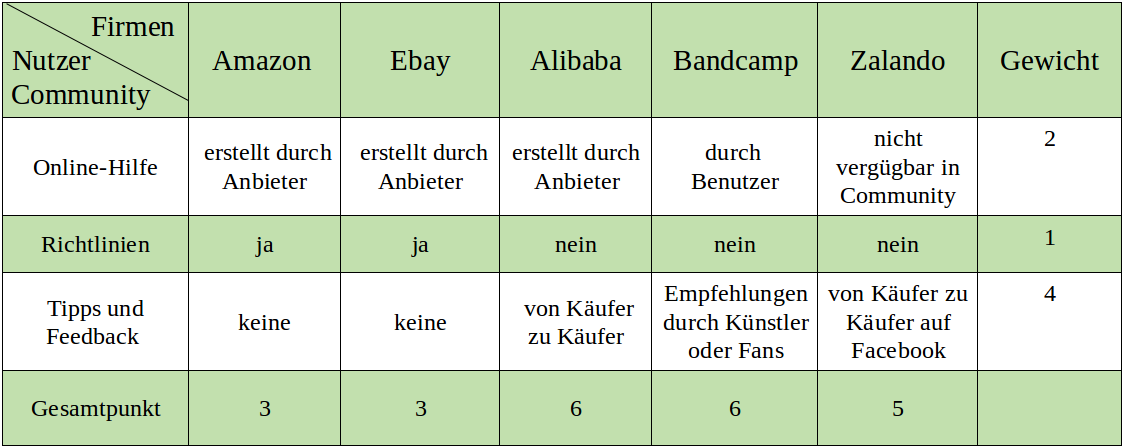
\includegraphics[width=1\textwidth]{bilder/tabelle-gruen.png}
	\caption{Nutzer-Community}
	\label{tab:tabelle-gruen}
\end{table}

In der Hinsicht bieten Alibaba und Bandcamp eine gute Plattform, sodass Nutzer miteinander kommunizieren können. Bei Alibaba geschieht dies durch ein separates Forum\footnote{Alibaba Community: \url{https://buyer.alibaba.com/forum}}. Bei Bandcamp\footnote{ Bandcamp Community: \url{https://bandcamp.com}} kann man sich nicht nur mit den Künstler verbinden, sondern auch mit anderen Fans Erfahrungen teilen.

Amazon\footnote{Amazon Community: \url{https://www.amazon.de/gp/help/customer/display.html?nodeId=201483620}} und Ebay\footnote{Ebay Community: \url{https://pages.ebay.de/help/policies/member-created-content-ov.html\#policy}} bieten auch Communities an. Deren Funktionen orientieren sich an der Online-Hilfe und Richtlinien. Es ist keine direkte Benutzerinteraktion verfügbar. Ein Ausnahme ist Zalando, die Firma betreibt ihre Community direkt auf Facebook\footnote{Zalando Community: \url{https://de-de.facebook.com/pg/Zalando.co.uk/community/}}.

\begin{figure}[htbp]
	\centering
	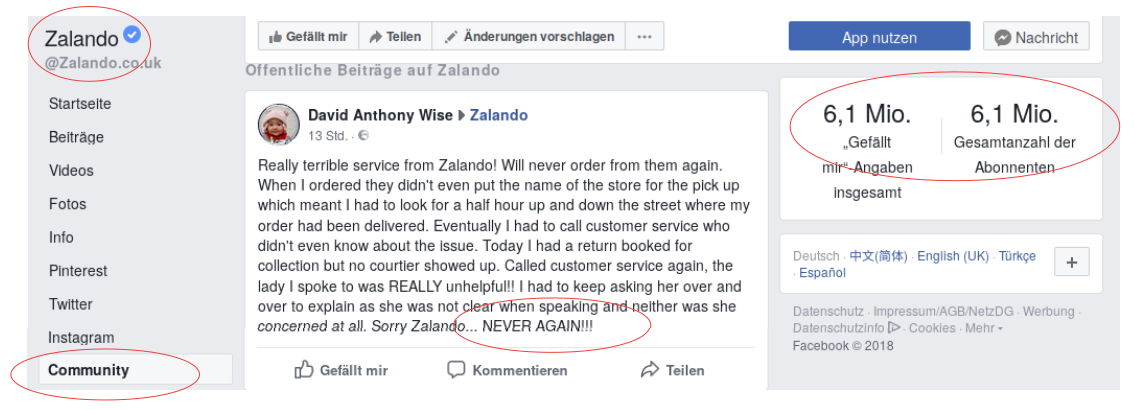
\includegraphics[width=1\textwidth]{bilder/zalando-community.png}
	\caption{Zalando Community auf Facebook}
	\label{fig:zalando-community}
\end{figure}

Wie in Abbildung \vref{fig:zalando-community} zu sehen, hat diese Maßnahme auch einige Nachteile. Z. B. muss man mit den Richtlinien von Facebook koexistieren. Zalando kann nicht die Kommentare kontrollieren. Ein weiter Nachteil ist, dass die schwerer für den Nutzer zu finden ist.


\section{Online Kommunikation}

Um die online Kommunikation von Webshops zu bewerten, wurden durch die Autorin die Kriterien Real-Time Chatten, Fotos senden und verfügbare Sprachkanäle ausgewählt. Das laut Meinung der Autorin primäre und wichtigste Kriterium ist hierbei, die Möglichkeit zum Real-Time Chatten. Fotos senden und zusätzliche Sprachkanäle spielen laut Meinung der Autorin eine untergeordnete Rolle.

Online Kommunikation (Real-Time Chatten) spielt für Webshops eine immer größere Rolle. Die Statistik von \textcite{aliyun}\footnote{Tochterfirma der Alibaba} zeigt, bis 12.2016 verwenden 100 Millionen Nutzer Aliwangwang. Dies ist eine spezielle Software für Real-Time Chatten und wird Hilfswerkzeug von Alibaba eingesetzt. Amazon unterstützt offensichtlich nicht diese Funktion. Zalando hat hierbei das gleiche Problem wie Amazon. Auf der Webseite von Zalando steht ebenfalls keine Echtzeit-Kommunikation zur Verfügung. \parencite{piatscheck}

Tabelle \vref{tab:tabelle-grau} stellt die Online Kommunikation der ausgewählten Webshops gegenüber.

\begin{table}[htbp]
	\centering
	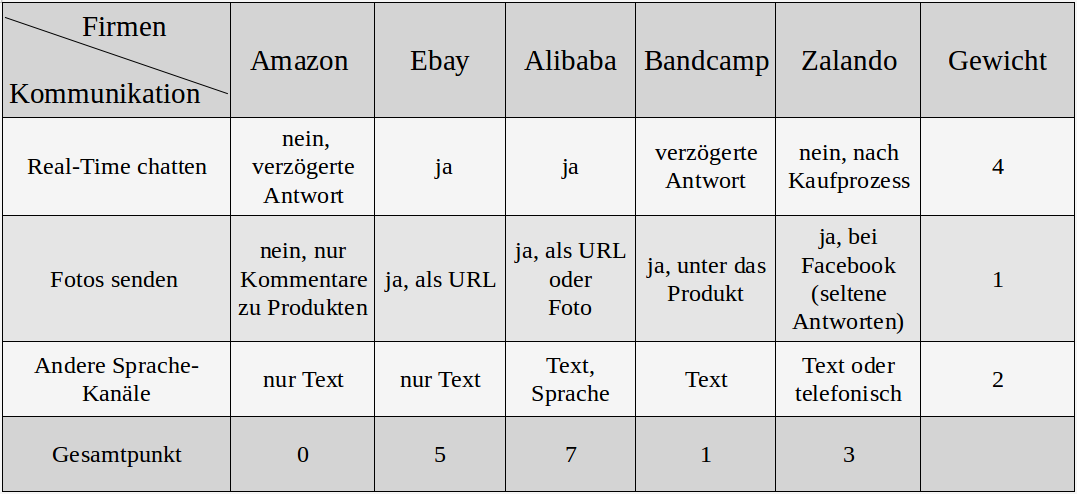
\includegraphics[width=1\textwidth]{bilder/tabelle-grau.png}
	\caption{Online Kommunikation}
	\label{tab:tabelle-grau}
\end{table}


\section{Produktvielfalt}

Viele Webshops orientiert sich bei ihrer Gründung auf eine bestimme Kundengruppe und auf eine bestimmte Geschäftsbeziehung. Am meisten verwendet werden die B2B , C2C und B2C Beziehungen. B2B steht für Business-to-Business und bezeichnet eine Handelsbeziehung, bei der Käufer und Verkäufer Unternehmen sind. B2C bedeutet Business-to-Consumer und bezieht sich auf Transaktionen zwischen Unternehmen (Anbieter) und Endkunden (Käufer). C2C bezeichnet ein Handel zwischen Kunden und Kunden.

Die Vielfalt der Produkte hat starken Einfluss auf den Umsatz. Nach einer Statistik von \textcite{statista} liegt Amazon auf dem 1. Platz und Zalando liegt auf den 3. Platz.

Nach obiger Statistik von \textcite{statista} wird bestätigt, dass der Gewinn abhängig von der Vielfalt der angebotenen Produkten ist. Nach der Meinung von Richard Lazazzera, How to Choose an Ecommerce Business Model\footnote{\url{https://www.shopify.com/blog/17240328-how-to-choose-an-ecommerce-business-model}} werden Businessmodelle unterschiedliche Kriterien unterteilt. Davon ist die Beziehung zwischen Käufer und Verkäufer die wichtigste. Danach belegen Marktpositionierung und Spezialisierung auf einen Produktbereich den zweiten Platz.

Tabelle \vref{tab:tabelle-rot} stellt die Geschäftsmodelle der ausgewählten Webshops gegenüber.

\begin{table}[htbp]
	\centering
	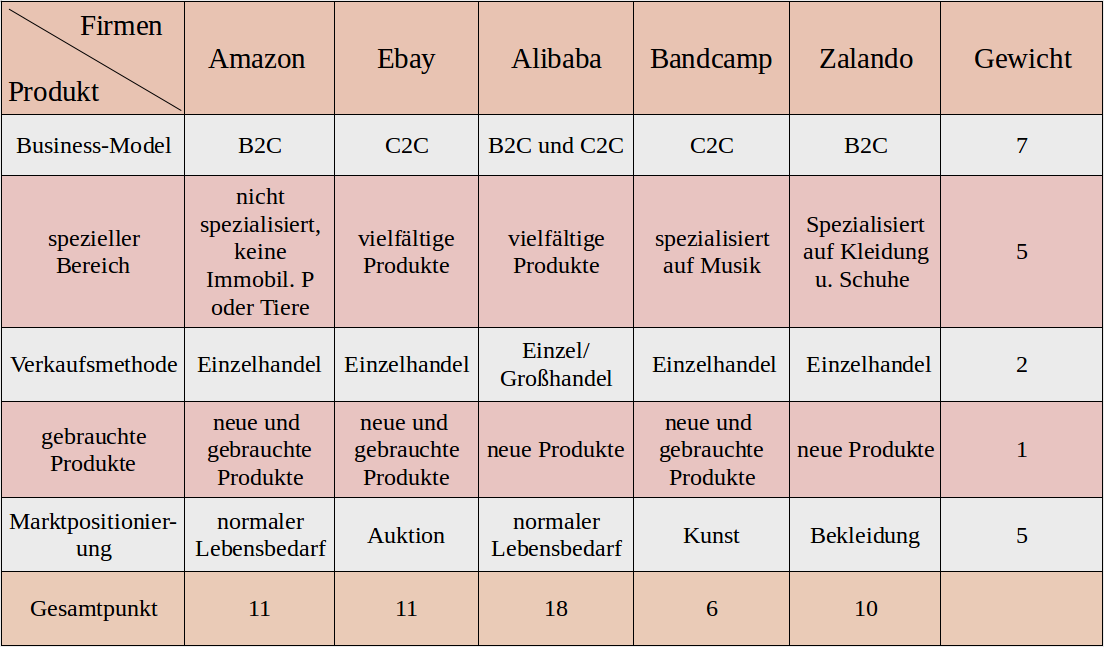
\includegraphics[width=1\textwidth]{bilder/tabelle-rot.png}
	\caption{Produktvielfalt}
	\label{tab:tabelle-rot}
\end{table}


\section{Zahlungsmethoden}

Weil Alibaba eine eigne Zahlungsmethode besitzt (Alipay - www.alipay.com), kann der Handelsbereich von Alibaba in den Finanzsektor erweitert werden. Unter der Prämisse die Sicherheit von Zahlungsinformation nicht zu verletzen haben Nutzer mehrere Möglichkeiten zu bezahlen. Andere Online Shops verwenden hierbei noch die Finanzprodukte von anderen Unternehmen, z.B. von Banken, PayPal usw. .

Um die Zahlungsmethoden von Webshops zu bewerten, wurden durch die Autorin die Zahlungsmöglichkeiten Kreditkarte, Giro-Karte, online Bezahldienste und eigne Finanzservices ausgewählt. Das laut Meinung der Autorin primäre und wichtigste Kriterium ist hierbei, die Möglichkeit \term{pay by others} zu nutzen. Bei den eigenen Finanzservices kann das Finanzprodukt durch den Provider selbst skaliert und gestaltet werden. Diese spielen aus diesem Grund laut Meinung der Autorin auch eine schwerwiegende Rolle.

Tabelle \vref{tab:tabelle-rot} stellt die Zahlungsmethoden der ausgewählten Webshops gegenüber.

\begin{table}[htbp]
	\centering
	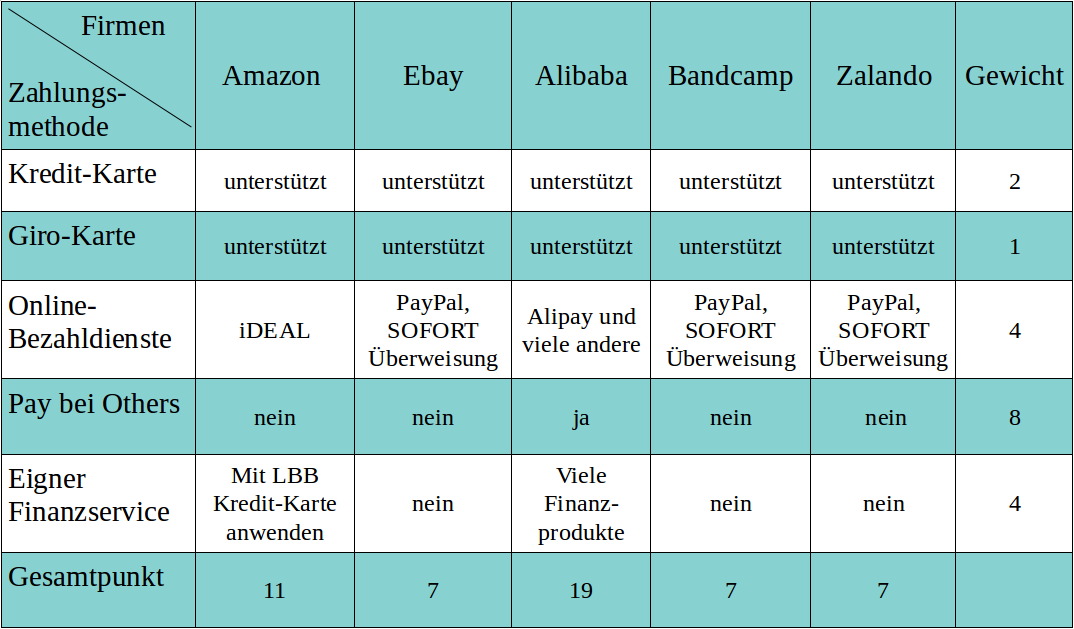
\includegraphics[width=1\textwidth]{bilder/tabelle-blau.png}
	\caption{Zahlungsmethoden}
	\label{tab:tabelle-blau}
\end{table}


\section{Methoden der Bewertung}

Bei der Bewertung bieten Amazon und Alibaba unterschiedliche Vorgehensweisen zum kommentieren an. So ist z. B. die Bewertung bei Amazon in Form von Sternen und einem Kommentar-Text realisiert. 1 bis 5 Sterne zeigen hier das Level der Zufriedenheit von unzufrieden bis sehr zufrieden. Abbildung \vref{fig:bewertung-amazon} zeigt Bewertungen in Amazon.

\begin{figure}[htbp]
	\centering
	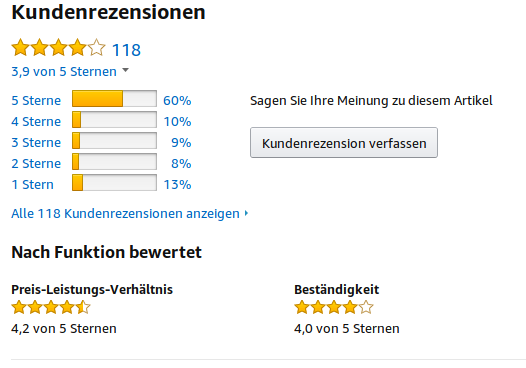
\includegraphics[width=1\textwidth]{bilder/bewertung-amazon.png}
	\caption{Bewertungen in Amazon}
	\label{fig:bewertung-amazon}
\end{figure}

Die rege Nutzung der Kommentare unter Produkten zeigt, immer mehrere Kunden wollen eine Bewertung abgeben, damit andere Nutzer Tipps oder Hinweise erhalten können. Die Webshops erstellen hierfür unterschiedliche Methoden, sodass die Bewertung konkreter und intuitiver sind. Nach der Meinung der Autorin sind diese zusätzlichen Methode für die Nutzer wichtig und nötig.

Tabelle \vref{tab:tabelle-gelb} stellt die Methoden der Bewertung für die ausgewählten Webshops gegenüber.

\begin{table}[htbp]
	\centering
	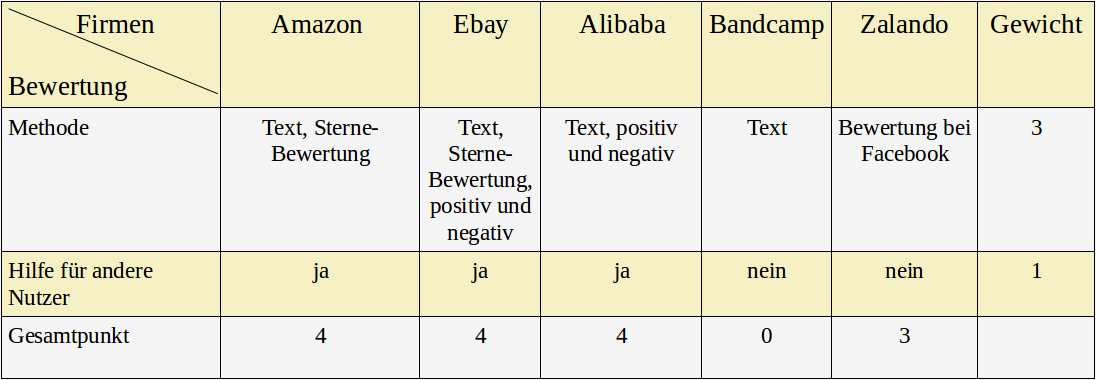
\includegraphics[width=1\textwidth]{bilder/tabelle-gelb.png}
	\caption{Methoden der Bewertung}
	\label{tab:tabelle-gelb}
\end{table}

\newpage


\section{Gesamtergebnis}

Tabelle \vref{tab:tabelle-ergebnis} stellt das Gesamtergebnis der ausgewählten Webshops gegenüber.

\begin{table}[htbp]
	\centering
	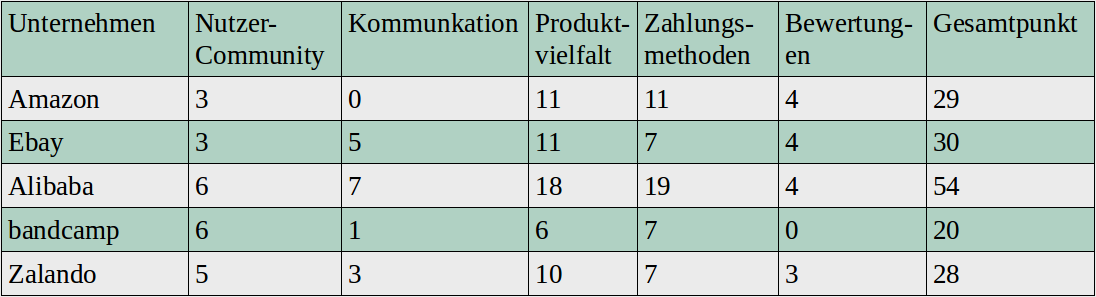
\includegraphics[width=1\textwidth]{bilder/tabelle-ergebnis.png}
	\caption{Gesamtergebnis}
	\label{tab:tabelle-ergebnis}
\end{table}

Nach der Berechnung des Gesamtergebnis können wir durch ein Diagramm zeigen, welcher Anbieter dominant ist. Abbildung \vref{fig:diagramm-ergebnis} stellt das Gesamtergebnis dar.

\begin{figure}[htbp]
	\centering
	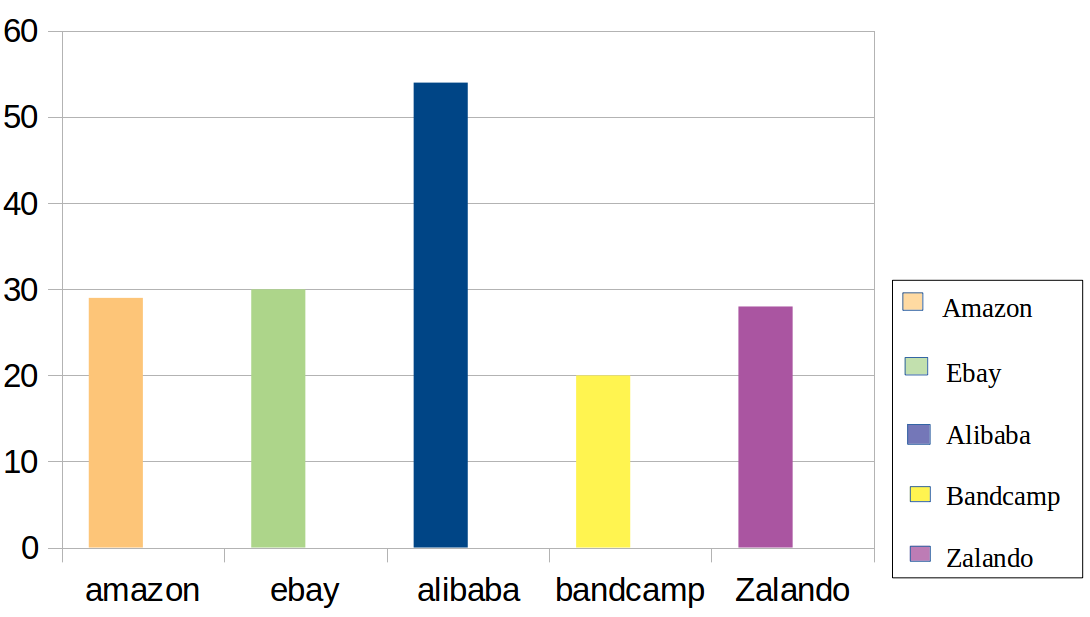
\includegraphics[width=0.7\textwidth]{bilder/diagramm-ergebnis.png}
	\caption{Auswertung Gesamtergebnis}
	\label{fig:diagramm-ergebnis}
\end{figure}

Das Diagramm zeigt als Ergebnis, dass im Vergleich zu anderen Firmen Alibaba die höchste Anzahl an Punkten erlangt hat. Der in dieser Arbeit zu konzipierende Shop soll die Vorteile von Alibaba aufgreifen und so die Servicequalität als Webshop weiter erhöhen.